\documentclass[preprint,12pt]{elsarticle}
\usepackage{fontspec}
\defaultfontfeatures{Ligatures=TeX}
\setmainfont{Times New Roman}
\setsansfont{Times New Roman}
\setmonofont{Courier New}
\usepackage{amsmath,amsthm,mathtools,unicode-math}
\setmathfont{STIX Two Math}
\usepackage{graphicx,booktabs,tabularx,xltabular,array,ragged2e}
\graphicspath{{figures/}}
\usepackage{caption,float,placeins,needspace}
\usepackage{lineno,setspace,microtype}
\usepackage{enumitem,xcolor}
\usepackage{algorithm}
\usepackage{algpseudocode}
\usepackage[hidelinks]{hyperref}
\hypersetup{pdftitle={Coordinate-Explicit and Route-Specific Finite-Precision Qualification of Tangent-Only Perturbations}}
\renewcommand{\tabularxcolumn}[1]{>{\RaggedRight\arraybackslash}p{#1}}
\renewcommand{\arraystretch}{1.14}
\captionsetup{font=small,labelfont=bf,skip=5pt}
\setlength{\parindent}{1.5em}
\setlength{\parskip}{0.08em}
\setlength{\emergencystretch}{2em}
\setstretch{1.04}
\newtheorem{proposition}{Proposition}
\newtheorem{corollary}{Corollary}
\theoremstyle{definition}
\newtheorem{definition}{Definition}
\journal{Computer Methods in Applied Mechanics and Engineering}

\begin{document}
\begin{frontmatter}

\title{Coordinate-Explicit and Route-Specific Finite-Precision Qualification of Tangent-Only Perturbations in Coupled Finite-Element Linearizations}
\author[aff1]{Bing Liang}
\author[aff1]{Yangqi Ma}
\author[aff1]{Weiji Sun\corref{cor1}}
\ead{sunweiji-1231@163.com}
\author[aff2]{Shi He}
\cortext[cor1]{Corresponding author.}
\address[aff1]{School of Mechanics and Engineering, Liaoning Technical University, No. 47 Zhonghua Road, Fuxin, Liaoning 123000, China}
\address[aff2]{China Coal Research Institute, Beijing 100013, China}

\begin{abstract}
Matrix norms and condition estimates quantify perturbation amplitude or worst-direction sensitivity, but they do not determine the response to one prescribed forcing direction or whether that response is distinguishable from finite-precision error. This study develops a coordinate-explicit, route-specific error-enclosure method for tangent-only perturbations in coupled finite-element linearizations. The method combines an exact finite-response identity, directional non-determination, coordinate covariance, and two a posteriori enclosures associated with distinct operation graphs: direct subtraction of parent solutions and solution of the response equation. Each enclosure covered 300/300 development systems and 300/300 newly generated holdout systems under both decimal-source and binary64-operand reference contracts. An independent 160-digit Decimal implementation checked 72 stratified lane comparisons with a maximum normalized difference of $6.96\times10^{-153}$. The response equation had lower reference error in 295/300 development and 271/300 new-holdout decimal-source cases, but no universal route ranking followed. Effectivity remained conservative. Its factorization showed median Frobenius-majorant inflation near $1.000$--$1.005$, whereas median directional-alignment inflation ranged from $1.36\times10^{3}$ to $2.31\times10^{4}$. Replication on two archived coupled finite-element tangents of dimensions 196 and 900 then demonstrated route-specific threshold qualification on application operators. The resulting procedure provides a reproducible reference benchmark for evaluating future scalable response estimators.
\end{abstract}

\begin{keyword}
tangent matrix \sep matrix perturbation \sep finite-element linearization \sep coordinate scaling \sep finite-precision error enclosure \sep directional response
\end{keyword}

\end{frontmatter}
\linenumbers

\section{Introduction}

Coupled nonlinear finite-element models repeatedly form block tangents whose unknowns carry different units and characteristic scales. Implementations may modify the matrix passed to a linear solver without adding the same term to the residual. We call this a \emph{tangent-only matrix perturbation}. Such a perturbation is distinct from residual-consistent stabilization and from a consistent algorithmic tangent, whose derivative must match the discrete constitutive update \cite{S32}. It is also distinct from inexact-Newton forcing, pseudo-transient continuation, conditioning-oriented finite-element reformulation, and preconditioning, which target nonlinear globalization, operator conditioning, or linear-solver performance rather than the response to one prescribed tangent modification \cite{S21,S29,S30,S31,S33,S34,S36}.

Classical diagnostics do not answer the complete selected-response question. A relative matrix norm measures perturbation amplitude in one representation; a condition estimate bounds worst-direction sensitivity; structured or componentwise conditioning describes admissible perturbation patterns; scaling changes the numerical coordinates; and verified or mixed-precision methods assess a prescribed solve \cite{S01,S02,S03,S05,S06,S07,S08,S11,S12,S13,S26,S28,S35,S37,S38,S39,S40,S41,S42,S43}. These tools remain indispensable, but neither matrix amplitude nor a worst-direction bound determines the realized action of $\Delta Jz$. A second distinction then appears in finite precision: the same exact response can be evaluated by subtracting two parent solutions or by solving its response equation, and the two operation graphs propagate different errors.

The computational advance developed here is the joint treatment of those two missing objects. The method first preserves the coordinate representation and selected forcing direction, then derives a posteriori finite-precision error enclosures for both operation graphs. The direct route propagates two parent-solve errors and subtraction error. The response route propagates the unperturbed-parent error, forcing-construction defect, and response-solve residual through the perturbed inverse. Consequently, route-specific intervals can be compared with a threshold without treating a matrix norm, a condition number, or raw route error as a substitute for the realized response.

Four contributions follow. First, Propositions~1--3 formalize the exact finite response, prove that matched matrix and worst-direction metrics do not determine a selected response, and distinguish coordinate covariance from same-numeric redeclaration. Second, Propositions~4 and 5 derive direct-difference and response-equation error enclosures, and Corollary~1 gives a sound threshold relation. Third, both enclosures are evaluated on a common 300-system development design and a newly generated 300-system holdout under decimal-source and binary64-operand reference contracts; an independent Decimal backend audits a stratified subset. Fourth, effectivity is decomposed into norm-majorant and directional-alignment inflation, then the complete procedure is replicated on two archived coupled finite-element tangents. The contribution is a reference-level response-enclosure method; sparse production estimation and controlled large-system cost validation remain a separate problem.

Table~\ref{tab:closest} identifies the object supplied beyond the closest computational contexts. Figure~\ref{fig:1} gives the method architecture, and Algorithms~\ref{alg:declaration}--\ref{alg:response} specify the two route implementations.

\begin{table}[htbp]
\centering
\footnotesize
\caption{Closest computational contexts and the response object supplied by this work.}
\label{tab:closest}
\begin{tabularx}{\linewidth}{>{\RaggedRight\arraybackslash}p{0.19\linewidth} >{\RaggedRight\arraybackslash}p{0.27\linewidth} >{\RaggedRight\arraybackslash}p{0.23\linewidth} X}
\toprule
Context & Primary object & Missing selected-response object & Supplied here \\
\midrule
Normwise and structured perturbation analysis & Matrix change and worst-case sensitivity & Realized action for one $b$ and $\Delta J$ & Directional response identity and non-determination result \\
Scaling and equilibration & Coordinate representation and conditioning & Same-operator versus redeclared-operator distinction & Coordinate-covariant perturbation contract \\
Residual-based or verified solve analysis & Error in one prescribed linear solve & Error propagation through two response operation graphs & Route-specific a posteriori enclosures \\
Newton regularization and continuation & Nonlinear or linear convergence behavior & Finite-precision response of one frozen tangent & Threshold-qualified local response only \\
\bottomrule
\end{tabularx}
\end{table}

\begin{figure}[H]
\centering

\includegraphics[width=0.98\linewidth,height=0.72\textheight,keepaspectratio]{F1_assessment_sequence.pdf}
\caption{Coordinate-explicit response-enclosure architecture. Matrix and inverse measures precede the selected response, after which the direct-difference and response-equation operation graphs produce separate finite-precision intervals. An external threshold gives above, below, or unresolved outcomes.}
\label{fig:1}
\end{figure}

Section~2 defines the response and algorithms. Sections~3 and 4 establish directional and coordinate properties. Section~5 derives and validates both error enclosures and analyzes their effectivity. Section~6 applies the method to two coupled finite-element linearizations, and Section~7 integrates the computational implications and scope.

\section{Mathematical and Computational Framework}

\subsection{Problem definition and solved-space contract}

Let $J$ and $J+\Delta J$ be square, nonsingular operators on one solved space, with a common right-hand side $b$ and one coordinate representation. A constrained problem enters only after its free or otherwise well-posed reduced space is specified. The vector norm and subordinate matrix norm are fixed together. The comparison therefore excludes changes in load, coordinates, nullspace, or residual root; under these assumptions the finite response identity has a single interpretation \cite{S02,S03}.

\subsection{Matrix, operator, and directional measures}

Let $z$, $z_g$, and $\delta z=z_g-z$ denote the unperturbed solution, perturbed solution, and response. The retained quantities answer separate questions: $\mu_J$ measures matrix amplitude; $\rho_1$ and $\rho_g$ measure first-order and finite worst-direction amplification; $\eta_z$ measures the selected response; $G_g$ compares that response with matrix amplitude; and $\kappa(J)$ measures normwise sensitivity. An operator norm is not a selected-probe response, and a condition number is not a mechanism classifier \cite{S01,S03}; the quantities form an assessment chain, not a composite score.

Figure~\ref{fig:2} places a tangent-only perturbation within a generic mixed-field block operator without assigning physical meaning to one scalar diagonal coefficient.

\begin{figure}[H]
\centering

\includegraphics[width=0.98\linewidth,height=0.72\textheight,keepaspectratio]{F2_mixed_field_tangent_anatomy.pdf}
\caption{Mixed-field tangent anatomy. (a) Coupled displacement, pressure, and saturation blocks carry distinct variable units. (b) A scalar identity perturbation in physical coordinates becomes field-scale dependent after coordinate transformation.}
\label{fig:2}
\end{figure}

Equation~\eqref{eq:framework_quantities} defines the solved systems and retained metrics. Table~\ref{tab:1} lists their roles and their non-substitution rules.

\begin{table}[htbp]
\centering
\small
\caption{Retained metrics and their non-substitution rules.}
\label{tab:1}
\begin{tabularx}{0.98\textwidth}{@{}>{\raggedright\arraybackslash}p{0.13\textwidth}>{\raggedright\arraybackslash}p{0.25\textwidth}XX@{}}
\toprule
\textbf{Metric} & \textbf{Definition} & \textbf{Question answered} & \textbf{Does not establish} \\
\midrule
$\mu_J$ & $\lVert\Delta J\rVert/\lVert J\rVert$ & Matrix-space amplitude & Realized response \\
$\rho_1$ & $\lVert J^{-1}\Delta J\rVert$ & First-order worst-direction amplification & Finite selected-probe response \\
$\rho_g$ & $\lVert(J+\Delta J)^{-1}\Delta J\rVert$ & Finite worst-direction amplification & Response for one right-hand side \\
$\eta_z$ & $\lVert z_g-z\rVert/\lVert z\rVert$ & Realized response for one probe & Worst-case behavior \\
$G_g$ & $\eta_z/\mu_J$ & Diagnostic response/amplitude ratio & Condition number or cause \\
$\kappa(J)\mu_J$ & $\lVert J\rVert\lVert J^{-1}\rVert\mu_J$ & Worst-case normwise comparison & Directional mechanism or trajectory \\
\bottomrule
\end{tabularx}
\par\vspace{2pt}\footnotesize\emph{Note:} Every metric requires a declared solved space, coordinates, compatible norm, right-hand side, perturbation route, and truth contract as applicable. Full declarations are listed in the Supplementary Information.

\end{table}

\begin{linenomath*}
\begin{equation}
\begin{aligned}
Jz &= b, & (J+\Delta J)z_g &= b, & \delta z &= z_g-z,\\
\mu_J &= \frac{\lVert\Delta J\rVert}{\lVert J\rVert}, &
\rho_1 &= \lVert J^{-1}\Delta J\rVert, &
\rho_g &= \lVert(J+\Delta J)^{-1}\Delta J\rVert,\\
\eta_z &= \frac{\lVert\delta z\rVert}{\lVert z\rVert}, &
G_g &= \frac{\eta_z}{\mu_J}\quad(\mu_J>0), &
\kappa(J) &= \lVert J\rVert\,\lVert J^{-1}\rVert .
\end{aligned}
\label{eq:framework_quantities}
\end{equation}
\end{linenomath*}

\subsection{Exact finite perturbation response}

\begin{proposition}[Exact finite response]
\label{prop:p1}
Let $J$ and $A=J+\Delta J$ be nonsingular, with $Jz=b$ and
$Az_g=b$. Then $\delta z=z_g-z$ satisfies
\begin{linenomath*}
\begin{equation}
\begin{aligned}
(J+\Delta J)\delta z &= -\Delta J z,\\
\delta z &= -(J+\Delta J)^{-1}\Delta J z.
\end{aligned}
\label{eq:finite_response_identity}
\end{equation}
\end{linenomath*}
No symmetry, definiteness, or small-perturbation assumption is required.
\end{proposition}

\begin{proof}
Substitution of $z_g=z+\delta z$ into $Az_g=b=Jz$ gives
$A\delta z=-\Delta Jz$. Nonsingularity of $A$ yields the second identity.
\end{proof}

The identity is classical perturbation algebra \cite{S02,S03}; its role here is to expose the realized forcing direction $\Delta Jz$ and the operator that propagates it. It is not itself a floating-point accuracy statement.

Equation~\eqref{eq:guarded_inverse_bound} follows from the subordinate norm and gives $\eta_z\leq\rho_g$ for nonzero $z$. This is a worst-direction bound, whereas $\eta_z$ evaluates only the direction generated by the selected solution and perturbation. Equality may occur under alignment but is not implied for an arbitrary right-hand side. The bound remains finite whenever the perturbed operator is nonsingular, even when the Neumann condition below is unavailable.

\begin{linenomath*}
\begin{equation}
\eta_z \leq \rho_g.
\label{eq:guarded_inverse_bound}
\end{equation}
\end{linenomath*}

Equation~\eqref{eq:neumann_bound} uses $E=J^{-1}\Delta J$, for which the response operator is $(I+E)^{-1}E$. If $\rho_1=\lVert E\rVert<1$, the Neumann series bounds the response by $\rho_1/(1-\rho_1)$. The denominator is essential; $\rho_1$ alone is only a first-order interpretation as $\rho_1\to0$. For $\rho_1\geq1$, Proposition~\ref{prop:p1} still holds for nonsingular matrices, but this Neumann argument provides no bound \cite{S02,S03}.

\begin{linenomath*}
\begin{equation}
\rho_1<1,\qquad
\eta_z \leq \frac{\rho_1}{1-\rho_1}.
\label{eq:neumann_bound}
\end{equation}
\end{linenomath*}

Equation~\eqref{eq:condition_comparison} records the submultiplicative estimate $\rho_1\leq\kappa(J)\mu_J$ in the same norm. If this product is below one, substitution in the Neumann result gives the stated finite comparison with its denominator. The estimate is coordinate-dependent, normwise, and worst case; it contains no information about the direction $\Delta Jz$. It can bound sensitivity under its assumptions but cannot identify the mechanism of one observed response \cite{S01,S03}.

\begin{linenomath*}
\begin{equation}
\begin{aligned}
\rho_1 &\leq \kappa(J)\mu_J,\\
\kappa(J)\mu_J<1 &\ \Longrightarrow\ 
\eta_z\leq\frac{\kappa(J)\mu_J}{1-\kappa(J)\mu_J}.
\end{aligned}
\label{eq:condition_comparison}
\end{equation}
\end{linenomath*}

Changing $b$ adds a data-perturbation term, and changing the residual or its root is not a tangent-only comparison. A singular unreduced operator first requires a well-posed quotient, projection, generalized inverse, or reduced formulation \cite{S17,S20}. Finally, the identities compare two local linear solves at one state; Newton acceptance, globalization, basin, and final root require separate nonlinear evidence \cite{S21,S23}.

\subsection{Computational assessment procedure}

Algorithms~\ref{alg:declaration}--\ref{alg:response} turn the mathematical contracts into two explicit computational graphs. The declaration stage freezes the solved space, coordinates, reference contract, and arithmetic specification. The direct graph propagates two parent-solve errors and subtraction error; the response graph propagates parent, forcing-construction, and response-solve errors. Section~\ref{sec:coordinate} establishes the transformation requirement, and Section~\ref{sec:error_enclosure} proves the corresponding enclosures.

\begin{algorithm}[H]
\caption{Coordinate and reference-problem declaration}
\label{alg:declaration}
\begin{algorithmic}[1]
\Require $J$, guarded operand $A$, declared perturbation $\Delta J$, $b$,
coordinate maps $D_x,D_r$, norm $\lVert\cdot\rVert$, computational route,
reference contract, arithmetic specification, and optional threshold $\tau$
\Ensure A frozen solved-space problem and the realized perturbation $E=A-J$
\State Restrict the system to the prescribed well-posed solved space
\State Transform $J$, $A$, $\Delta J$, and $b$ consistently with $D_x,D_r$
\State Set $E\gets A-J$ in the selected reference contract
\State Check dimensions, finiteness, operand identity, and reference-contract separation
\State Freeze the route, precision, norm, threshold, and output fields before evaluation
\end{algorithmic}
\end{algorithm}

\begin{algorithm}[H]
\caption{Direct-difference finite-precision error enclosure}
\label{alg:direct}
\begin{algorithmic}[1]
\Require Frozen output of Algorithm~\ref{alg:declaration}
\Ensure $\widetilde\delta_{\rm d}$, $U_{\rm d}$, $[L_{\rm d},H_{\rm d}]$
\State Compute $\widetilde z\approx J^{-1}b$ and
$\widetilde z_g\approx A^{-1}b$
\State Form $r_z=b-J\widetilde z$ and
$r_{z_g}=b-A\widetilde z_g$
\State Obtain majorants $\beta_J\geq\lVert J^{-1}\rVert_2$ and
$\beta_A\geq\lVert A^{-1}\rVert_2$
\State Set $U_z\gets\beta_J\lVert r_z\rVert_2$ and
$U_{z_g}\gets\beta_A\lVert r_{z_g}\rVert_2$
\State Compute $\widetilde\delta_{\rm d}\gets
\operatorname{fl}(\widetilde z_g-\widetilde z)$ and its subtraction bound
$U_{\rm sub}$
\State Set $U_{\rm d}\gets U_z+U_{z_g}+U_{\rm sub}$
\State Set $d_{\rm d}\gets\lVert\widetilde\delta_{\rm d}\rVert_2$,
$L_{\rm d}\gets\max(0,d_{\rm d}-U_{\rm d})$, and
$H_{\rm d}\gets d_{\rm d}+U_{\rm d}$
\State Report the relation of $[L_{\rm d},H_{\rm d}]$ to $\tau$
\end{algorithmic}
\end{algorithm}

\begin{algorithm}[H]
\caption{Response-equation finite-precision error enclosure}
\label{alg:response}
\begin{algorithmic}[1]
\Require Frozen output of Algorithm~\ref{alg:declaration}
\Ensure $\widetilde\delta_{\rm r}$, $U_{\rm r}$, $[L_{\rm r},H_{\rm r}]$
\State Compute $\widetilde z\approx J^{-1}b$ and
$r_z=b-J\widetilde z$
\State Obtain $\beta_J\geq\lVert J^{-1}\rVert_2$,
$\beta_A\geq\lVert A^{-1}\rVert_2$, and
$\alpha_E\geq\lVert E\rVert_2$; set
$U_z\gets\beta_J\lVert r_z\rVert_2$
\State Construct the route operand
$\widetilde f\gets\operatorname{fl}(-\Delta J\widetilde z)$
\State Compute $\widetilde\delta_{\rm r}\approx A^{-1}\widetilde f$
\State Form $q_f=\widetilde f+E\widetilde z$ and
$r_\delta=\widetilde f-A\widetilde\delta_{\rm r}$
\State Set
$U_{\rm parent}\gets\beta_A\alpha_EU_z$,
$U_{\rm force}\gets\beta_A\lVert q_f\rVert_2$, and
$U_{\rm solve}\gets\beta_A\lVert r_\delta\rVert_2$
\State Set
$U_{\rm r}\gets U_{\rm parent}+U_{\rm force}+U_{\rm solve}$
\State Set $d_{\rm r}\gets\lVert\widetilde\delta_{\rm r}\rVert_2$,
$L_{\rm r}\gets\max(0,d_{\rm r}-U_{\rm r})$, and
$H_{\rm r}\gets d_{\rm r}+U_{\rm r}$
\State Report the relation of $[L_{\rm r},H_{\rm r}]$ to $\tau$
\end{algorithmic}
\end{algorithm}


The architecture is not an arbitrary checklist. Table~\ref{tab:necessity} links each component to a specific omission exposed by the existing evidence. The conclusions are intentionally local: they establish what is needed to interpret one selected response, not prevalence across operator populations.

\begin{table}[htbp]
\centering
\small
\caption{Evidence-backed necessity of the assessment components.}
\label{tab:necessity}
\input{T2_component_necessity_v0.10.0.tex}
\end{table}

\FloatBarrier
\section{Analytical Verification}

\begin{proposition}[Directional non-determination]
\label{prop:p2}
For every $\varepsilon>0$, there exist two perturbations with identical
$\mu_J$, $\rho_1$, $\rho_g$, and $\kappa_2(J)$ but different realized
responses $\eta_z$. Hence those scalar matrix and worst-direction quantities
do not determine the response for a selected right-hand side.
\end{proposition}

\noindent\textit{Construction and proof.}
Fix the Euclidean vector norm and spectral matrix norm, take $J=I_2$, and choose the first coordinate as the right-hand side. Two rank-one diagonal perturbations with the same amplitude $\varepsilon$ act respectively along and orthogonally to the unperturbed solution. Equation~\eqref{eq:p2_construction} isolates direction while holding the operator, norm, right-hand side, perturbation amplitude, and condition number fixed.

\begin{linenomath*}
\begin{equation}
\begin{aligned}
J&=I_2, & b&=e_1=[1,0]^{\mathsf T},\\
\Delta J_A&=\varepsilon\,\operatorname{diag}(1,0), &
\Delta J_B&=\varepsilon\,\operatorname{diag}(0,1), & \varepsilon&>0.
\end{aligned}
\label{eq:p2_construction}
\end{equation}
\end{linenomath*}

The matrix and operator metrics are matched in the two cases. Since $\lVert J \rVert=1$, both perturbations give $\mu_J = \varepsilon$; since $J^{-1}=I_2$, both give $\rho_1 = \varepsilon$; and since the guarded inverse scales only the perturbed coordinate, both give $\rho_g = \varepsilon/(1+\varepsilon)$. The spectral condition number is one in each case. Thus even the combination of matrix amplitude, unguarded inverse amplification, guarded inverse amplification, and condition number is identical. This equality is stronger than matching only $\lVert \Delta J \rVert$: the two perturbations also have the same finite worst-direction bound. What remains unspecified by those metrics is whether the selected solution lies in the range of the perturbation. The construction therefore prepares a direct test of whether matched matrix-level and operator-level quantities determine one realized response.

\begin{linenomath*}
\begin{equation}
\begin{aligned}
\mu_J(A)&=\mu_J(B)=\varepsilon,\\
\rho_1(A)&=\rho_1(B)=\varepsilon,\\
\rho_g(A)&=\rho_g(B)=\frac{\varepsilon}{1+\varepsilon},\\
\kappa_2(J)&=1.
\end{aligned}
\label{eq:p2_matched_metrics}
\end{equation}
\end{linenomath*}

Equation~\eqref{eq:p2_matched_metrics} shows that the constructions have identical matrix amplitude, inverse-mediated measures, and condition number. Their realized responses nevertheless separate. In case A, the perturbation acts on $z=e_1$, giving $\eta_z=\varepsilon/(1+\varepsilon)$ and attaining the guarded-inverse bound. In case B, $\Delta J_Bz=0$, so the guarded and unguarded solutions coincide and $\eta_z=0$. The missing information is directional alignment between the solution, perturbation range, and propagated response. This proves Proposition~\ref{prop:p2}.

Figure~\ref{fig:3} contrasts the aligned and orthogonal constructions under matched matrix and worst-direction quantities.

\begin{figure}[H]
\centering

\includegraphics[width=0.98\linewidth,height=0.72\textheight,keepaspectratio]{F3_directional_response.pdf}
\caption{Directional counterexample. Alignment geometry separates the selected probe from the perturbation range; matrix and worst-direction quantities remain matched while the realized response differs for six pre-specified perturbation amplitudes.}
\label{fig:3}
\end{figure}

\begin{linenomath*}
\begin{equation}
\eta_z(A)=\frac{\varepsilon}{1+\varepsilon},
\qquad \eta_z(B)=0.
\label{eq:p2_realized_response}
\end{equation}
\end{linenomath*}

Equation~\eqref{eq:p2_realized_response} records the exact directional separation used in the numerical reproduction.

The pre-specified numerical reproduction evaluated six frozen amplitudes from $1\allowbreak\times10^{-12}$ to $1\allowbreak\times10^{-2}$ using an independent high-precision route for the exact construction. Across all six rows, the maximum relative difference between the paired matrix metrics was $0$, the maximum relative error in the nonzero aligned response was $8.721173782511926\allowbreak\times10^{-102}$, and the maximum absolute orthogonal response was $0$. The implementation check summarized in Eq.~\eqref{eq:p2_reproduction_accuracy} reproduces the analytical metric match and the response distinction without changing the construction after observation. The numerical verification validates implementation of this exact example; it does not add an empirical frequency statement. In particular, six amplitudes for one two-dimensional construction are not an operator-family survey, and the zero response in case B follows from exact orthogonality rather than from a general perturbation-screening rule.

\begin{linenomath*}
\begin{equation}
\begin{aligned}
\max \delta_{\mathrm{matched}} &= 0,\\
\max \delta_{\eta_A} &= 8.721173782511926\times10^{-102},\\
\max |\eta_B| &= 0.
\end{aligned}
\label{eq:p2_reproduction_accuracy}
\end{equation}
\end{linenomath*}

Proposition~\ref{prop:p2} is an existence result rather than a frequency statement. The numerical reproduction verifies the implementation of its exact construction; the synthetic-family and finite-element evidence below address separately designed operator sets.

\FloatBarrier
\section{Coordinate-Transformation Verification}
\label{sec:coordinate}

\begin{proposition}[Coordinate covariance and redeclaration non-equivalence]
\label{prop:p3}
Under $z=D_x\widehat z$ and $\widehat r=D_r^{-1}r$, one fixed
perturbed operator transforms as
$\widehat J=D_r^{-1}JD_x$ and
$\widehat{\Delta J}=D_r^{-1}\Delta JD_x$. A same-numeric perturbation
redeclared after the coordinate change is generally a different physical
operator.
\end{proposition}

Let the physical unknown and scaled unknown be related by the nonsingular matrix $D_x$, and let residual coordinates be transformed by the nonsingular matrix $D_r$. The frozen convention is $z = D_x \widehat z$ and $\widehat r = D_r^{-1} r$. Substitution into $r = Jz-b$ defines the scaled operator and right-hand side as $\widehat J = D_r^{-1} J D_x$ and $\widehat b = D_r^{-1}b$. A perturbation belongs to the same operator relation and must therefore transform as $\widehat{\Delta J} = D_r^{-1} \Delta J D_x$. Equation~\eqref{eq:coordinate_transform} defines equivalent coordinates only when the unknown, residual, right-hand side, operator, and perturbation are transformed together. Applying a transformation to some objects while independently redefining another object creates a different perturbed problem, even if the same numeric symbol is displayed. Scaling and equilibration literature motivates explicit coordinate declarations but does not supply unique physical choices for $D_x$ and $D_r$ \cite{S05,S06,S07,S08}.

\begin{linenomath*}
\begin{equation}
\begin{aligned}
z&=D_x\widehat z, & \widehat r&=D_r^{-1}r,\\
\widehat J&=D_r^{-1}JD_x, & \widehat b&=D_r^{-1}b,\\
\widehat{\Delta J}&=D_r^{-1}\Delta J D_x.
\end{aligned}
\label{eq:coordinate_transform}
\end{equation}
\end{linenomath*}

Suppose first that the perturbation is declared in physical coordinates as $\Delta J_{\mathrm{phys}} = \varepsilon I$. Equation~\eqref{eq:physical_identity_transform} gives its representation in the scaled operator is obtained by the joint transformation, giving $\widehat{\Delta J} = \varepsilon D_r^{-1}D_x$. The transformed perturbation is a scalar identity only when $D_r^{-1}D_x$ is a scalar multiple of the identity, and it retains the same $\varepsilon I$ representation only when $D_x = D_r$. In a mixed-dimensional system, different unknown and residual scales generally make the diagonal entries field dependent. This is a coordinate statement: it identifies the scaled representation of one fixed physical operator. It neither changes that operator nor evaluates the practical consequences of its action. Treating the transformed matrix as if it had to retain the original scalar identity form would replace transformation by redeclaration.

\begin{linenomath*}
\begin{equation}
\Delta J_{\mathrm{phys}}=\varepsilon I,
\qquad \widehat{\Delta J}=\varepsilon D_r^{-1}D_x.
\label{eq:physical_identity_transform}
\end{equation}
\end{linenomath*}

The reverse construction begins with a perturbation declared in scaled coordinates as $\widehat{\Delta J} = \beta I$. Equation~\eqref{eq:scaled_identity_mapping} maps it to physical coordinates and gives $\Delta J_{\mathrm{phys}} = \beta D_r D_x^{-1}$, which is generally a field-dependent diagonal operator. Thus a dimensionless identity guard denotes a family of physical perturbations indexed by the declared unknown and residual scales. The mapping does not select those scales; it only states which physical operator corresponds to the scaled identity after the coordinate contract is fixed. Consequently, the label $\beta I$ is incomplete without the operator space, $D_x$, $D_r$, and the direction in which the transformed solution is interpreted. This distinction also prevents a same-numeric identity written in two coordinate systems from being treated as one perturbation without checking the transformation rule.

Figure~\ref{fig:4} distinguishes equivalent coordinate transformation from same-numeric-label redeclaration.

\begin{figure}[H]
\centering

\includegraphics[width=0.98\linewidth,height=0.72\textheight,keepaspectratio]{F4_coordinate_transformation.pdf}
\caption{Coordinate transformation versus operator redeclaration. Consistent transformation preserves the represented perturbation, whereas reusing a same-numeric identity in scaled coordinates maps back to a different physical perturbation.}
\label{fig:4}
\end{figure}

\begin{linenomath*}
\begin{equation}
\widehat{\Delta J}=\beta I,
\qquad \Delta J_{\mathrm{phys}}=\beta D_rD_x^{-1}.
\label{eq:scaled_identity_mapping}
\end{equation}
\end{linenomath*}

The equivalent-transformation calculation used a two-dimensional construction with pre-specified scale factors $1$, $10$, $1\allowbreak\times10^{3}$, and $1\allowbreak\times10^{6}$. In the equivalent transformed-operator route, the unknown, right-hand side, operator, and perturbation were transformed consistently. The resulting maximum relative difference between physical-equivalent perturbation operators was $7.490674676829096\allowbreak\times10^{-102}$, and the relative spread of the physical response was $0$. The check in Eq.~\eqref{eq:p3_reproduction_accuracy} validates the implemented transformation for the frozen construction and pre-specified scales. They do not establish that arbitrary independently specified guards are invariant; invariance here follows because the transformed descriptions represent the same physical operator and the same physical solution response. The numerical values therefore check the algebraic mapping rather than define a coordinate-independent scalar guard.

\begin{linenomath*}
\begin{equation}
\begin{aligned}
\max \delta_{\mathrm{operator}} &= 7.490674676829096\times10^{-102},\\
\operatorname{spread}(\eta_z)_{\mathrm{transformed}} &= 0.
\end{aligned}
\label{eq:p3_reproduction_accuracy}
\end{equation}
\end{linenomath*}

The second pre-specified lane reapplied the same numeric identity after changing coordinates instead of transforming the original perturbation. With $D_r=I_2$ and $D_x=\operatorname{diag}(1,s)$, that scaled identity maps back to a physical perturbation whose second diagonal entry is $\varepsilon/s$, whereas the original physical identity retains $\varepsilon$ on both diagonal entries. The two physical perturbations coincide at $s=1$ and differ for every pre-specified $s>1$; the pre-specified inequality check was therefore true. Equation~\eqref{eq:p3_redeclaration_result} demonstrates that a shared numeric label does not establish operator equivalence. It does not show that one of the resulting operators should be selected. The observed response change follows from comparing different physical perturbations, not from a failure of coordinate transformation.

\begin{linenomath*}
\begin{equation}
\Delta J_{\mathrm{redeclared}}\neq
\Delta J_{\mathrm{transformed}}\quad\text{for every pre-specified }s>1.
\label{eq:p3_redeclaration_result}
\end{equation}
\end{linenomath*}

Proposition~\ref{prop:p3} is a covariance requirement, not a scale-selection rule. Equilibration and physical nondimensionalization may pursue different objectives \cite{S07,S08}; the present result requires only that an operator comparison preserve its declared coordinates or explicitly acknowledge a redeclared perturbation.

\FloatBarrier
\section{Finite-Precision Error-Enclosure Method and Validation}
\label{sec:error_enclosure}

\subsection{Two computational routes}

Let $A=J+E$ denote the guarded operand in one fixed reference contract.
The exact parent and response problems are
\begin{linenomath*}
\begin{equation}
Jz=b,\qquad Az_g=b,\qquad A\delta z=-Ez,
\qquad \delta z=z_g-z.
\label{eq:route_exact_problems}
\end{equation}
\end{linenomath*}
Here $E=A-J$ is the realized perturbation of the two solve operands. The
declared $\Delta J$ remains the operand used by the floating-point
forcing construction. This distinction is immaterial when addition is exact,
but retains last-bit operand effects when $A$ and $J$ are captured
independently under IEEE~754 binary arithmetic \cite{S09,S10}.

The direct route computes two parent solutions and subtracts them,
\begin{linenomath*}
\begin{equation}
\widetilde\delta_{\rm d}
=\operatorname{fl}(\widetilde z_g-\widetilde z)
=\delta z+e_g-e+q_{\rm sub},
\label{eq:direct_operation_graph}
\end{equation}
\end{linenomath*}
where $e=\widetilde z-z$, $e_g=\widetilde z_g-z_g$, and
$q_{\rm sub}$ is the subtraction error.

\begin{proposition}[Direct-difference error enclosure]
\label{prop:p4}
If $\lVert e\rVert_2\leq U_z$,
$\lVert e_g\rVert_2\leq U_{z_g}$, and
$\lVert q_{\rm sub}\rVert_2\leq U_{\rm sub}$, then
\begin{linenomath*}
\begin{equation}
\lVert\widetilde\delta_{\rm d}-\delta z\rVert_2
\leq U_{\rm d}:=U_z+U_{z_g}+U_{\rm sub}.
\label{eq:direct_difference_enclosure}
\end{equation}
\end{linenomath*}
\end{proposition}

\begin{proof}
Subtract $\delta z$ from Eq.~\eqref{eq:direct_operation_graph} and apply
the triangle inequality.
\end{proof}

The response route constructs
$\widetilde f=\operatorname{fl}(-\Delta J\widetilde z)$ and solves
$A\widetilde\delta_{\rm r}\approx\widetilde f$. Define the forcing
defect $q_f=\widetilde f+E\widetilde z$ and response residual
$r_\delta=\widetilde f-A\widetilde\delta_{\rm r}$.

\begin{proposition}[Response-equation error enclosure]
\label{prop:p5}
Assume $\lVert\widetilde z-z\rVert_2\leq U_z$ and let
$\beta_A\geq\lVert A^{-1}\rVert_2$ and
$\alpha_E\geq\lVert E\rVert_2$. Then
\begin{linenomath*}
\begin{equation}
\begin{aligned}
\lVert\widetilde\delta_{\rm r}-\delta z\rVert_2
&\leq U_{\rm r},\\
U_{\rm r}
&:=\underbrace{\beta_A\alpha_EU_z}_{U_{\rm parent}}
+\underbrace{\beta_A\lVert q_f\rVert_2}_{U_{\rm force}}
+\underbrace{\beta_A\lVert r_\delta\rVert_2}_{U_{\rm solve}}.
\end{aligned}
\label{eq:response_equation_enclosure}
\end{equation}
\end{linenomath*}
\end{proposition}

\begin{proof}
Because $A\delta z=-Ez$ and
$A\widetilde\delta_{\rm r}=\widetilde f-r_\delta$,
\[
A(\widetilde\delta_{\rm r}-\delta z)
=q_f-E(\widetilde z-z)-r_\delta .
\]
Multiplication by $A^{-1}$, submultiplicativity, and the assumed majorants
give Eq.~\eqref{eq:response_equation_enclosure}.
\end{proof}

Propositions~\ref{prop:p4} and \ref{prop:p5} enclose the same exact
response through different operation graphs. Their components therefore
cannot be exchanged merely because the observed response vectors are close.

\subsection{Parent bounds, threshold relation, and reference contracts}

For a computed solution $\widetilde x$ of $Bx=c$, residual
$r=c-B\widetilde x$, and any
$\beta_B\geq\lVert B^{-1}\rVert_2$, the parent error satisfies
\begin{linenomath*}
\begin{equation}
\lVert\widetilde x-x\rVert_2
\leq\lVert B^{-1}\rVert_2\lVert r\rVert_2
\leq\beta_B\lVert r\rVert_2.
\label{eq:parent_majorant}
\end{equation}
\end{linenomath*}
The implementation uses
\begin{linenomath*}
\begin{equation}
\beta_B=\lVert B^{-1}\rVert_F\geq\lVert B^{-1}\rVert_2,
\qquad
\alpha_E=\lVert E\rVert_F\geq\lVert E\rVert_2.
\label{eq:frobenius_majorants}
\end{equation}
\end{linenomath*}
Thus the Frobenius quantities are explicit majorants; they are not
subordinate matrix norms paired with the Euclidean vector norm.
For binary64 subtraction, the adopted allowance is
\begin{linenomath*}
\begin{equation}
U_{\rm sub}
=\gamma_1\lVert|\widetilde z_g|+|\widetilde z|\rVert_2
+\sqrt n\,2^{-1075},\qquad
\gamma_1=\frac{2^{-53}}{1-2^{-53}}.
\label{eq:subtraction_allowance}
\end{equation}
\end{linenomath*}

For either route $a\in\{\mathrm d,\mathrm r\}$, let
$d_a=\lVert\widetilde\delta_a\rVert_2$ and let $U_a$ be the matching
enclosure. The response-magnitude interval is
\begin{linenomath*}
\begin{equation}
L_a=\max(0,d_a-U_a),\qquad H_a=d_a+U_a.
\label{eq:response_magnitude_interval}
\end{equation}
\end{linenomath*}

\begin{corollary}[Sound threshold relation]
\label{cor:threshold}
If Proposition~\ref{prop:p4} or \ref{prop:p5} applies, then
$L_a\leq\lVert\delta z\rVert_2\leq H_a$. Hence, for a threshold
$\tau\geq0$ fixed independently of the observed response,
$L_a>\tau$ proves that the exact response exceeds $\tau$, and
$H_a<\tau$ proves that it lies below $\tau$.
\end{corollary}

\begin{definition}[Route-qualified threshold relation]
The outcome is \emph{above} if $L_a>\tau$, \emph{below} if
$H_a<\tau$, and \emph{unresolved} otherwise. Setting $\tau=0$ recovers
zero exclusion as a special case.
\end{definition}

Two reference contracts are retained. The decimal-source contract treats the
registered decimal matrices and vectors as the real-valued problem. The
binary64-operand contract reconstructs the captured IEEE operands exactly and
treats those values as a separate real-valued problem. Each residual,
inverse majorant, forcing defect, and reference response is evaluated only
within its matching contract. Figure~\ref{fig:5} shows both reference lanes
and both operation graphs.

\begin{figure}[H]
\centering

\includegraphics[width=0.98\linewidth,height=0.72\textheight,keepaspectratio]{F5_two_reference_contracts.pdf}
\caption{Reference-contract and operation-graph anatomy. Decimal-source and binary64-operand problems remain separate. Within either contract, direct subtraction combines two parent and subtraction components, whereas the response equation combines parent propagation, forcing construction, and response-solve components.}
\label{fig:5}
\end{figure}

\subsection{Prospective enclosure validation}

The direct-route model was first evaluated on a 300-system development set
and a disjoint 300-system holdout containing SPD, nonsymmetric, and
saddle-point-like matrices of dimensions $2$, $4$, $8$, and $16$. Each
reference contract achieved 300/300 coverage on both sets. A subsequent
preregistered response-route study froze Proposition~\ref{prop:p5} and then
generated a new 300-system holdout with disjoint seeds, condition exponents,
and perturbation amplitudes. Both routes were evaluated without changing the
matrices or gates.

Table~\ref{tab:routevalidation} reports the result. Direct and response
enclosures each covered 300/300 errors in all four data-set--contract
combinations. The development decimal-source response error was lower in
295/300 cases, reproducing the earlier route comparison; the corresponding
count was 271/300 on the new holdout. In the binary64-operand contract, the
counts were 199/300 and 160/300. Lower response error therefore did not imply
a universal route ordering.

\begin{table}[htbp]
\centering
\footnotesize
\caption{Prospective direct- and response-route enclosure validation. Coverage is shown as covered/total; the last two columns count cases in which the response route produced the smaller quantity.}
\label{tab:routevalidation}
\begin{tabularx}{\linewidth}{>{\RaggedRight\arraybackslash}p{0.16\linewidth} >{\RaggedRight\arraybackslash}p{0.16\linewidth} *{4}{>{\centering\arraybackslash}X}}
\toprule
Set & Reference contract & Direct coverage & Response coverage & Lower response error & Lower response enclosure \\
\midrule
Development & Decimal source & 300/300 & 300/300 & 295/300 & 283/300 \\
Development & Binary64 operand & 300/300 & 300/300 & 199/300 & 229/300 \\
New holdout & Decimal source & 300/300 & 300/300 & 271/300 & 229/300 \\
New holdout & Binary64 operand & 300/300 & 300/300 & 160/300 & 188/300 \\
\bottomrule
\end{tabularx}

\end{table}

The 120- and 180-digit core evaluations agreed to maximum normalized
differences of $5.16\times10^{-110}$ on development and
$6.82\times10^{-107}$ on the new holdout, with no coverage-decision
mismatch. A separately implemented 160-digit Python Decimal solver, using
manual elimination and importing neither NumPy, SciPy, nor mpmath, checked
36 stratified holdout systems in both contracts. Its 72 lane comparisons
agreed with maximum normalized difference $6.96\times10^{-153}$. The first
execution and two tooling-only comparator corrections are retained in the
Supplement rather than overwritten.

\subsection{Effectivity anatomy}

Coverage alone does not measure sharpness. For positive true route error
$e_a=\lVert\widetilde\delta_a-\delta z\rVert_2$, define
$I_a=U_a/e_a$. For a parent solve whose bound is
$U=\lVert B^{-1}\rVert_F\lVert r\rVert_2$ and whose true error is
$e=\lVert B^{-1}r\rVert_2$, the effectivity factorizes exactly as
\begin{linenomath*}
\begin{equation}
I_{\rm parent}
=\underbrace{\frac{\lVert B^{-1}\rVert_F}
{\lVert B^{-1}\rVert_2}}_{\text{norm-majorant inflation}}
\underbrace{\frac{\lVert B^{-1}\rVert_2\lVert r\rVert_2}
{\lVert B^{-1}r\rVert_2}}_{\text{directional-alignment inflation}}.
\label{eq:effectivity_factorization}
\end{equation}
\end{linenomath*}
This decomposition connects enclosure conservativeness to the same
worst-direction versus realized-direction distinction established by
Proposition~\ref{prop:p2}.

Across 2,400 parent records, the median norm-majorant factor was
$1.0001$ on development and $1.0050$ on the original holdout. Median
directional inflation instead ranged from $1.18\times10^4$ to
$2.31\times10^4$ on development and from $1.36\times10^3$ to
$1.88\times10^3$ on holdout (Table~\ref{tab:anatomy}). The central
conservativeness therefore came primarily from replacing the realized
residual direction by a worst-direction inverse norm, not from using the
Frobenius norm instead of the spectral norm.

\begin{table}[htbp]
\centering
\footnotesize
\caption{Factorization of parent-bound effectivity. Ranges span both parent systems and both reference contracts.}
\label{tab:anatomy}
\begin{tabularx}{\linewidth}{>{\RaggedRight\arraybackslash}p{0.18\linewidth} >{\RaggedRight\arraybackslash}p{0.25\linewidth} *{2}{>{\centering\arraybackslash}X}}
\toprule
Set & Quantity & Median range & 95th-percentile range \\
\midrule
Development & Frobenius majorization & $1.0001$--$1.0001$ & $1.94$--$1.94$ \\
Development & Directional inflation & $1.18\times10^{4}$--$2.31\times10^{4}$ &
$3.18\times10^{8}$--$8.53\times10^{8}$ \\
Original holdout & Frobenius majorization & $1.0050$--$1.0050$ & $2.69$--$2.69$ \\
Original holdout & Directional inflation & $1.36\times10^{3}$--$1.88\times10^{3}$ &
$3.59\times10^{7}$--$8.72\times10^{7}$ \\
\bottomrule
\end{tabularx}

\end{table}

A main-effects model for $\log_{10}I_{\rm eff}$ used condition exponent,
$\log_{10}\epsilon$, $\log_2n$, matrix family, and reference lane. The
development fit gave adjusted $R^2=0.869$ and drop-one partial
$R^2=0.855$ for condition exponent. The original holdout fit gave adjusted
$R^2=0.057$ and condition partial $R^2=0.029$. Conditioning was therefore
dominant in the development design but did not transfer as a universal
importance law. The largest finite direct-route ratio is reported as
$\log_{10}I_{\rm eff}=86.90$; it arises from a
$4.9995\times10^{-102}$ reference error rather than from undercoverage.
The exact value and case identifier remain in the machine-readable record.

\begin{figure}[H]
\centering
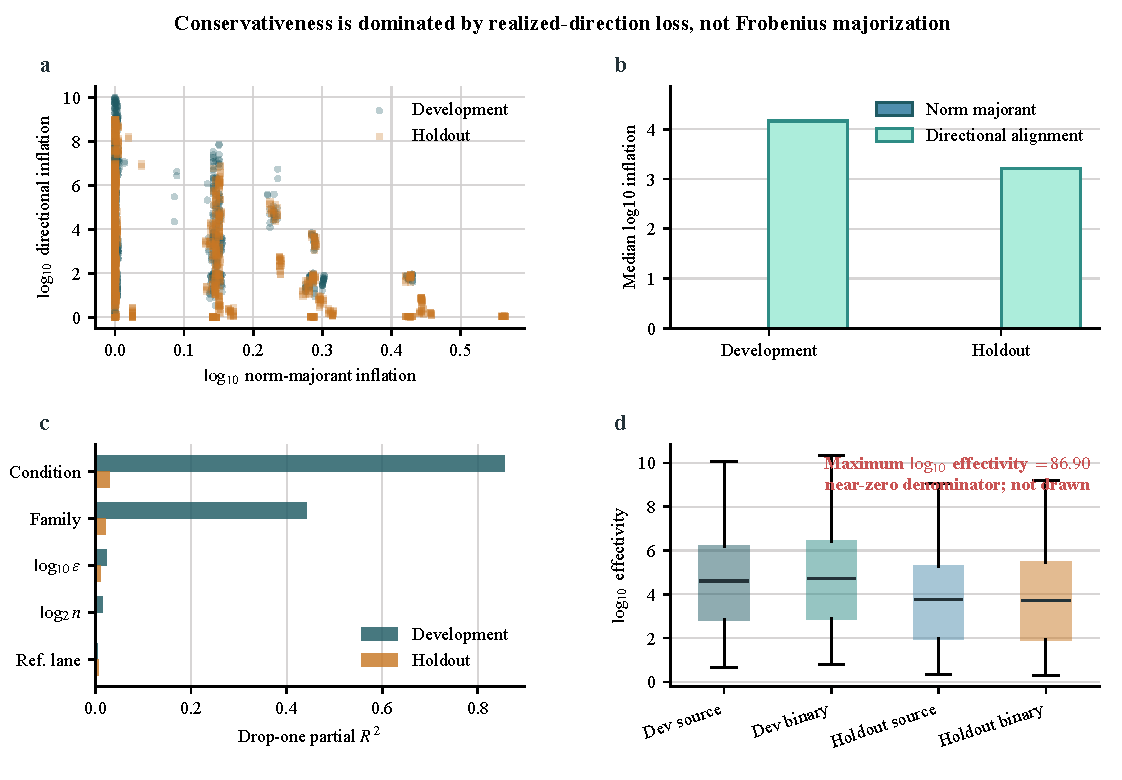
\includegraphics[width=0.98\linewidth,height=0.72\textheight,keepaspectratio]{F6_effectivity_dependence.pdf}
\caption{Effectivity anatomy and finite-grid attribution. (a) Norm-majorant inflation remains near unity while directional inflation spans orders of magnitude. (b) Median factor ranges for development and holdout. (c) Drop-one partial $R^2$ values from registered main-effects models. (d) Direct-route effectivity versus condition exponent, including the near-zero-denominator extreme. Partial contributions are non-additive.}
\label{fig:6}
\end{figure}

\subsection{Route comparison after enclosure validation}

Figure~\ref{fig:7} joins raw arithmetic behavior to valid enclosure
consequences. In the decimal-source contract, the median response-to-direct
error ratio was $5.29\times10^{-8}$ on development and
$2.01\times10^{-3}$ on the new holdout; the median bound ratio was
$6.90\times10^{-8}$ and $4.11\times10^{-3}$, respectively. In the
binary64-operand contract, median error ratios were $0.631$ and $0.980$,
with median bound ratios $0.462$ and $0.480$. The response graph thus
reduced both error and enclosure in many cases, but its effectivity remained
conservative and some cases favored the direct route.

\begin{figure}[H]
\centering
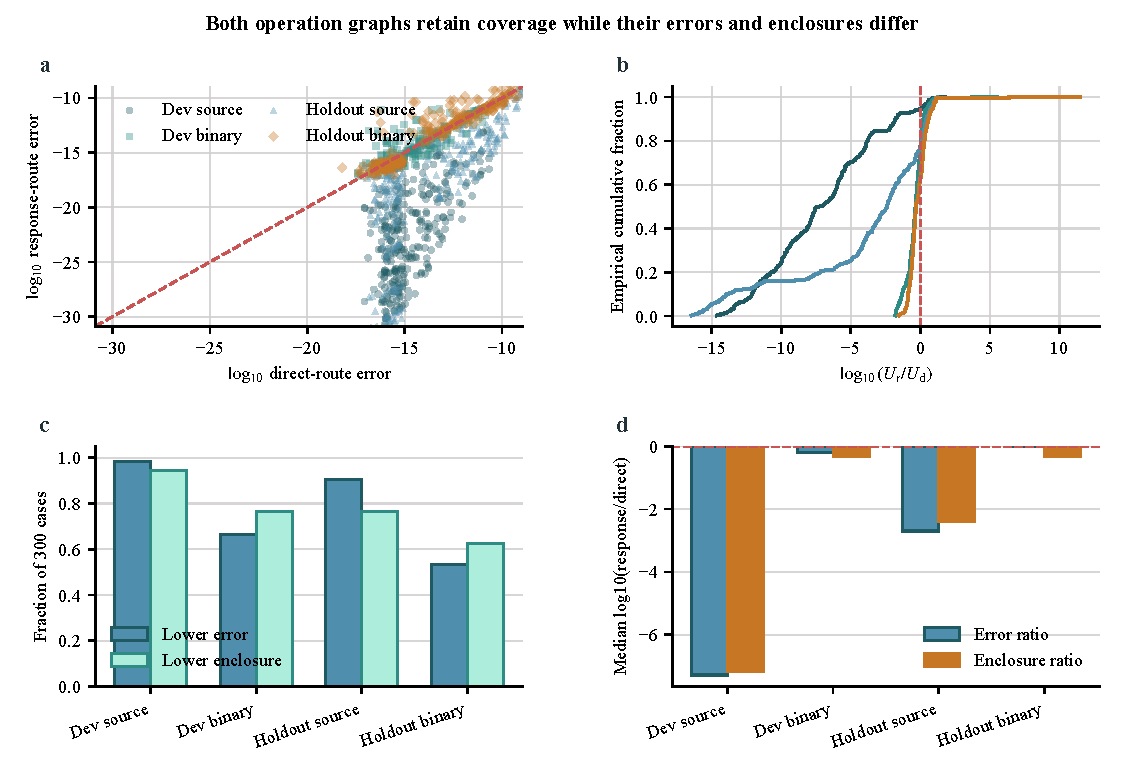
\includegraphics[width=0.98\linewidth,height=0.72\textheight,keepaspectratio]{F7_route_error_mechanism.pdf}
\caption{Validated route comparison. (a) Response- versus direct-route reference error. (b) Distribution of $U_{\rm r}/U_{\rm d}$. (c) Cases with lower response-route error and enclosure. (d) Median error and enclosure ratios by data set and reference contract. Both routes retain complete coverage; the figure does not assert universal superiority.}
\label{fig:7}
\end{figure}

The validation establishes conditional finite-precision enclosures for the
registered finite grids. It does not make them interval-arithmetic
certificates, calibrated probabilistic intervals, or scalable sparse
estimators. Those distinctions are consolidated here rather than repeated
after each positive result.


\FloatBarrier

\section{Applications to Two Coupled Finite-Element Linearizations}
\label{sec:applications}

\subsection{Archived operator snapshots and reference construction}

The application stage uses two independently archived transformed free-system snapshots from a four-field displacement--pressure--saturation discretization. M8 contains 324 total nodal degrees of freedom and 196 free unknowns; M16 contains 1156 and 900, respectively. The free ordering retains 49 and 225 coordinates for each of $u_x$, $u_y$, $p$, and $S$. Unknown scales are $10^{-5}$ for both displacement components, $10^7$ for pressure, and $10^{-1}$ for saturation. Table~\ref{tab:feprovenance} records the corresponding matrix sizes and sparsity.

\begin{table}[htbp]
\centering
\footnotesize
\caption{Provenance and coordinate content of the archived finite-element tangents. Each per-field count applies to $u_x$, $u_y$, $p$, and $S$.}
\label{tab:feprovenance}
\begin{tabularx}{\linewidth}{>{\centering\arraybackslash}p{0.08\linewidth} >{\centering\arraybackslash}p{0.15\linewidth} >{\centering\arraybackslash}p{0.15\linewidth} >{\centering\arraybackslash}p{0.14\linewidth} X}
\toprule
Case & Total / free DOFs & Free DOFs per field & Stored nonzeros & Unknown-coordinate scales \\
\midrule
M8 & 324 / 196 & 49 & 5,442 &
$u:10^{-5}$, $p:10^{7}$, $S:10^{-1}$ \\
M16 & 1,156 / 900 & 225 & 28,259 &
$u:10^{-5}$, $p:10^{7}$, $S:10^{-1}$ \\
\bottomrule
\end{tabularx}

\end{table}

Each snapshot fixes the IEEE binary64 matrices $J$ and $A$, common right-hand side $b$, free-degree-of-freedom ordering, unknown and residual scales, and Euclidean comparison norm before either route is evaluated. The realized perturbation $E=A-J$ is diagonal in both cases. M8 and M16 are independently captured states rather than a controlled mesh or condition sequence.

For each case, the reference problem is the real-valued system represented exactly by the captured binary64 operands. Integer-ratio reconstruction, signed-zero checks, and the elementwise identity $A=J+E$ establish that operand contract. Parent systems and the response equation are solved independently at 120 and 180 decimal digits. Each observed response is compared only with the error enclosure for its own operation graph.

\subsection{Case results and offline cost}

For M8, the maximum normalized 120/180-digit difference is $8.81\times10^{-121}$ and the maximum reference relative residual is $2.55\times10^{-124}$. Direct subtraction gives $d_{\mathrm{obs}}=2.919\times10^{-12}$ with $U=5.880\times10^{-13}$; the response equation gives $d_{\mathrm{obs}}=2.920\times10^{-12}$ with $U=2.588\times10^{-22}$. Both intervals lie above the special threshold $\tau=0$.

For M16, the maximum normalized precision difference is $3.97\times10^{-121}$ and the maximum reference relative residual is $4.14\times10^{-124}$. Direct subtraction gives $d_{\mathrm{obs}}=2.463\times10^{-11}$ with $U=3.971\times10^{-12}$; the response equation gives $d_{\mathrm{obs}}=2.464\times10^{-11}$ with $U=6.930\times10^{-21}$. Again, both route-specific intervals lie above $\tau=0$. Rounded route, precision, and component summaries appear in Supplementary Tables~S6--S8; exact decimal strings remain in the machine-readable ledgers.

\begin{figure}[H]
\centering

\includegraphics[width=0.98\linewidth,height=0.72\textheight,keepaspectratio]{F8_two_operator_route_qualification.pdf}
\caption{Route-specific response intervals for two independently archived coupled finite-element tangents. The left panels show matrix sparsity; the right panels show direct-difference and response-equation intervals on case-specific scales. Dashed references denote $\tau=0$.}
\label{fig:8}
\end{figure}

\begin{table}[htbp]
\centering
\footnotesize
\caption{Route-specific response intervals for the two finite-element tangents at $\tau=0$. Displayed values are rounded; Supplementary Table~S4 retains exact strings.}
\label{tab:3}

\resizebox{\linewidth}{!}{%
\begin{tabular}{@{}llrrrrrl@{}}
\toprule
\textbf{Case} & \textbf{Dimension} & \textbf{Route} & \textbf{Observed response} & \textbf{Uncertainty bound} & \textbf{Lower bound} & \textbf{Rel.-error upper bound} & \textbf{Decision} \\
\midrule
M8 & 196 & Direct difference & $2.918501\times 10^{-12}$ & $5.880138\times 10^{-13}$ & $2.330488\times 10^{-12}$ & $2.523136\times 10^{-1}$ & Distinguishable \\
M8 & 196 & Response equation & $2.920014\times 10^{-12}$ & $2.588300\times 10^{-22}$ & $2.920014\times 10^{-12}$ & $8.863996\times 10^{-11}$ & Distinguishable \\
M16 & 900 & Direct difference & $2.463376\times 10^{-11}$ & $3.970800\times 10^{-12}$ & $2.066296\times 10^{-11}$ & $1.921699\times 10^{-1}$ & Distinguishable \\
M16 & 900 & Response equation & $2.463672\times 10^{-11}$ & $6.930483\times 10^{-21}$ & $2.463672\times 10^{-11}$ & $2.813071\times 10^{-10}$ & Distinguishable \\
\bottomrule
\end{tabular}%
}

\end{table}

The complete M8 reference calculation, including both precision levels and an independent repeat, required approximately 468~s and 110~MiB of peak memory. M16 required 10.4~h and 1.35~GiB. These measurements define the implementation as a reproducible reference benchmark against which scalable estimators can be tested; two timings do not constitute a complexity fit.

\FloatBarrier
\section{Discussion}

\subsection{The computational object beyond matrix diagnostics}

The method addresses a question that matrix amplitude and conditioning leave
open. The quantities $\mu_J$, $\rho_1$, $\rho_g$, and $\kappa(J)$ quantify
representation-dependent change or worst-direction sensitivity. They do not
identify whether the selected solution activates the perturbation range.
Proposition~\ref{prop:p2} makes that information deficit exact: all four
matrix-level quantities can be matched while the realized response changes
from the guarded-inverse bound to zero. Structured and componentwise
conditioning sharpen the admissible perturbation model
\cite{S39,S40,S41}, but a selected response still requires the direction
$Ez$ and its propagation by $A^{-1}$.

The second advance concerns computation of that response. Direct subtraction
and the response equation are algebraically equivalent in exact arithmetic,
yet they form different finite-precision operation graphs.
Propositions~\ref{prop:p4} and \ref{prop:p5} provide separate a posteriori
error enclosures for those graphs. This is the central difference from a
generic verified solve: the solve-error ingredients are propagated to a
specific perturbation-response object, and the forcing-construction defect is
retained when the declared perturbation and realized solve operands differ at
the last bit. The threshold relation in Corollary~\ref{cor:threshold} then
turns the enclosed response into an above, below, or unresolved result without
using a condition number as a surrogate decision.

\subsection{Why the enclosures are conservative}

Complete coverage and useful sharpness are different properties. The
effectivity factorization in Eq.~\eqref{eq:effectivity_factorization}
localizes the dominant source of conservativeness. Median inflation caused by
the Frobenius majorant was almost unity, whereas replacing the realized
residual direction by the worst inverse direction contributed median factors
between $1.36\times10^3$ and $2.31\times10^4$. The large central ratios are
therefore not primarily a Frobenius-versus-spectral artifact; they arise
because a valid normwise residual bound discards directional alignment.

The multivariable analysis also prevents overinterpreting a single marginal
correlation. Condition exponent explained most registered variation in the
development design, but its drop-one partial $R^2$ fell from $0.855$ to
$0.029$ on the original holdout. Matrix family, perturbation amplitude, and
reference lane likewise changed importance across the two finite grids. The
data support a mechanism---worst-direction replacement can be highly
conservative---but not a universal effectivity scaling law. The extreme
$\log_{10}I_{\rm eff}=86.90$ further illustrates why ratios become
unstable when the true error approaches zero even though absolute coverage
remains valid.

\subsection{What the two routes reveal}

The response equation reduced decimal-source reference error in 295/300
development cases and 271/300 new-holdout cases. Its enclosure was also
smaller in 283/300 and 229/300 cases. Binary64-operand comparisons were less
separated: the response route had lower error in 199/300 development and
160/300 holdout cases, and lower bounds in 229/300 and 188/300. These
differences are consistent with the operation graphs. Direct subtraction can
lose small responses between two complete parent solutions; the response
equation avoids that subtraction but inherits forcing-construction and
response-solve errors. The new result is not that one graph always wins, but
that both can now be compared through valid route-specific enclosures rather
than raw arithmetic error alone.

\subsection{Computational-mechanics meaning and scope}

For a frozen coupled tangent, the method answers whether the correction
induced by a tangent-only modification is above, below, or unresolved with
respect to an independently supplied response threshold. A solver developer
may connect that threshold to an accepted Newton-correction tolerance, a
residual scale, an energy norm, or a quantity-of-interest budget. Such a
choice converts a vague statement that the matrix change is \emph{small}
into a testable statement about the selected correction at one nonlinear
state. M8 and M16 demonstrate this chain for
displacement--pressure--saturation operators with explicit field scales; both
operation graphs excluded the special threshold zero.

The present implementation is intentionally a high-precision reference
benchmark. It does not select a perturbation, prove nonlinear convergence,
or certify an engineering model. It is also not an outward-rounded interval
solver. Sparse estimation, controlled large-system sequences, blind transfer,
and coverage--tightness--cost validation belong to a separate scalable-method
study. Consolidating these limits here preserves the positive result: a
coordinate-consistent, operation-graph-specific response can be enclosed and
independently checked before a production estimator is judged against it.


\FloatBarrier

\section{Conclusions}

This study formulated tangent-only perturbation assessment as a selected
finite-response problem rather than a matrix-magnitude test. Exact algebra
separates the represented perturbation, worst-direction amplification, and
realized forcing direction, while coordinate covariance prevents a
same-numeric diagonal from being mistaken for the same operator after
rescaling.

The main computational result is a pair of a posteriori finite-precision error
enclosures for two algebraically equivalent but arithmetically distinct
operation graphs. The direct enclosure propagates two parent-solve errors and
subtraction error; the response enclosure propagates parent error,
forcing-construction defect, and response-solve residual. Each route covered
300/300 development and 300/300 newly generated holdout systems in both
reference contracts. An independent Decimal implementation confirmed a
stratified 72-lane subset to $6.96\times10^{-153}$ normalized agreement.

The analysis also explains why coverage can coexist with conservative bounds.
Frobenius majorization contributed median factors near unity, whereas
directional-alignment inflation contributed factors of $10^3$--$10^4$.
The response graph often reduced both arithmetic error and enclosure size, but
the binary64 and holdout results ruled out a universal route ranking.

Application to 196- and 900-dimensional coupled finite-element tangents showed
that the full coordinate--response--enclosure chain can qualify archived
application operators. The resulting implementation is a reproducible
reference benchmark for future sparse estimators, not a replacement for their
independent coverage, tightness, and cost validation.


\section*{Data availability}
The non-confidential frozen operands, synthetic validation records, exact-value tables, claim--evidence matrix, and provenance files supporting this study are archived in Zenodo at \href{https://doi.org/10.5281/zenodo.21870862}{https://doi.org/10.5281/zenodo.21870862} \cite{liang2026artifact}. This version-specific DOI identifies the v1.1.0 release used in the present study. The archive excludes Abaqus executables, user-element source, solver state histories, and engineering project data.

\section*{Code availability}
The scripts for the analytical constructions, finite-precision error-enclosure validation, and the two reference finite-element linearization applications are available at \href{https://github.com/yqma7980/scale-explicit-matrix-perturbation-observability}{https://github.com/yqma7980/scale-explicit-matrix-perturbation-observability} and are preserved with the cited Zenodo release. Code is licensed under the MIT License; data and documentation are licensed under CC BY 4.0.

\section*{Reproducibility statement}
The reported calculations use immutable operand snapshots, explicit coordinates and reference problems, two independent precision levels, independent-process repeatability checks, and exact output records. The Supplementary Information retains full numerical precision, error-enclosure components, and execution provenance.

\section*{CRediT authorship contribution statement}
\textbf{Bing Liang:} Conceptualization, Methodology, Formal analysis, Writing -- original draft, Writing -- review and editing, Supervision. \textbf{Yangqi Ma:} Methodology, Software, Validation, Formal analysis, Investigation, Data curation, Visualization, Writing -- original draft, Writing -- review and editing. \textbf{Weiji Sun:} Conceptualization, Methodology, Resources, Supervision, Project administration, Funding acquisition, Writing -- review and editing. \textbf{Shi He:} Methodology, Validation, Writing -- review and editing.

\section*{Funding}
This work was supported by the National Natural Science Foundation of China (General Program, Grant No. 52474038, awarded to Weiji Sun).

\section*{Declaration of competing interest}
The authors declare that they have no known competing financial interests or personal relationships that could have appeared to influence the work reported in this paper.

\section*{Declaration of generative AI and AI-assisted technologies in the manuscript preparation process}
During preparation of this work, the authors used Codex (OpenAI desktop version 26.730.8199.0; Codex CLI version 0.145.0) to assist with organizing and formatting the LaTeX manuscript source. After using this tool, the authors reviewed and edited the manuscript as needed and take full responsibility for the content of the publication.

\bibliographystyle{elsarticle-num}
\bibliography{Paper2_references_v0.13.0}

\end{document}
